\documentclass[fullscreen=true, bookmarks=true, hyperref={pdfencoding=unicode}]{beamer}
\usepackage[utf8]{inputenc}                                % Кодировка
\usepackage[english,russian]{babel}                        % Переносы
\usepackage{xcolor}                                        % Работа с цветом
\usepackage{amsmath,amssymb,amsfonts}                      % Символы АМО
\usepackage{graphicx}                                      % Графика
\usepackage[labelsep=period]{caption}                      % Разделитель в подписях к рисункам и таблицам
\usepackage{hhline}                                        % Для верстки линий в таблицах
\usepackage{tikz}                                          % Для простых рисунков в документе
\usepackage{fancybox}                                      % Пакет для отрисовки рамок
\usepackage{verbatim}                                      % Для вставки кода в презентацию
\usepackage{animate}                                       % Для вставки видео в презентацию
\usepackage{xmpmulti}                                      % Для вставки gif в презентацию
\usepackage{multirow}
\usepackage{mathrsfs}
\usepackage[normalem]{ulem}

\usetikzlibrary{arrows, snakes, backgrounds}                 % Для отрисовки стрелок
\usetikzlibrary{positioning, fit, arrows.meta, shapes, calc}
% used to avoid putting the same thing several times...
% Command \empt{var1}{var2}
\newcommand{\empt}[2]{$#1^{\langle #2 \rangle}$}

\graphicspath{{images/}}                                   % Путь до рисунков
\setbeamertemplate{caption}[numbered]                      % Включение нумерации рисунков

\definecolor{links}{HTML}{2A1B81}                          % blue for url links
\hypersetup{colorlinks,linkcolor=,urlcolor=links}          % nothing for others

\usetheme{boxes}
\usecolortheme{crane}

\usepackage{pythonhighlight}

\newtheorem*{question}{Вопрос}

\title{Лекция 10. Ранжирование и рекомендательные системы}
\author{Александр Юрьевич Авдюшенко}
\institute{МКН СПбГУ}
\date{21 апреля 2022}
\titlegraphic{
\includegraphics[keepaspectratio,width=0.5\textwidth]{logo_fmkn.png}}


\begin{document}
%\unitlength=2mm

% выводим заглавие
\begin{frame}
\transdissolve[duration=0.2]
\titlepage
\end{frame}


\begin{frame}
  \frametitle{Пятиминутка}
  \begin{itemize}
    \item Какие типы зависимостей выделяют во временных рядах?
    \item Опишите парой предложений на идейном уровне модель прогнозирования ARIMA
    \item Что такое «гетероскедастичность»?
  \end{itemize}
\end{frame}


\begin{frame}
  \frametitle{Ранжирование (learning to rank)}

  $X$ — множество объектов

  $X^\ell = \{x_1, \dots, x_\ell\}$ — обучающая выборка

  $i \prec j$ — правильный порядок на парах $(i, j) \in \{1, \dots, \ell\}^2$

  \vspace{1cm}
  {\bf Задача:}

  построить ранжирующую функцию $a: X \to \mathbb{R}$ такую, что

  $i \prec j \Rightarrow a(x_i) < a(x_j)$
\end{frame}


\begin{frame}
  \frametitle{Источники правильных ответов}

  \begin{columns}
      \begin{column}{.5\paperwidth}
        \begin{center}
          
\includegraphics[keepaspectratio,
                           width=.45\paperwidth]{asessor-yandex.jpg}
        \end{center}
      \end{column}
      \begin{column}{.5\paperwidth}
        \begin{center}
          
\includegraphics[keepaspectratio,
                           width=.45\paperwidth]{department_review.jpg}
        \end{center}
      \end{column}
  \end{columns}

\end{frame}


\begin{frame}
  \frametitle{Примеры задач ранжирования}

  {\bf Поисковая система}

  $x_i$ — (запрос, $i$-ый документ)

  \pause
  \vspace{1cm}
  {\bf Социальная сеть}

    $x_i$ — (пользователь, $i$-ая единица контента)
\end{frame}


\begin{frame}
  \frametitle{Факторы ранжирования в социальной сети}

  {\bf Пользователь}
  \begin{itemize}
    \item возраст, пол и т.д.
    \item content-based описание (TF-IDF, тематическое моделирование, embeddings)
    \item проявленные интересы (группы, подписки)
  \end{itemize}
  \pause
  {\bf Контент}
  \begin{itemize}
    \item content-based описание(TF-IDF, тематическое моделирование, embeddings)
    \item проявленная заинтересованность к данному контенту
    \item рейтинг/популярность автора контента или самого контента (ссылки, лайки)
  \end{itemize}
  \pause
  {\bf Общие}
  \begin{itemize}
    \item повестка дня
    \item время суток
  \end{itemize}
\end{frame}


\begin{frame}
  \frametitle{Content-based факторы. TF-IDF}

  {\bf TF-IDF} (Term Frequency - Inverse Document Frequency)

  Например, переводим {\bf текст} в $[\text{tfidf}(w_1), \dots, \text{tfidf}(w_k)]$

  $$ \text{tfidf}(w_i) = \text{tf}_i \cdot \text{idf}_i = \text{tf}_i \cdot \log{\frac{N}{N_i}} $$

  $ \text{tf}_i = \frac{n_i}{\sum\limits_j n_j} $ — частота $i$-ого слова в тексте,

  $N$ — число текстов, $N_i$ — число текстов с данным словом
\end{frame}


\begin{frame}
  \frametitle{Content-based факторы}
  \framesubtitle{напоминание}

  \begin{block}{Тематическое моделирование}
    Тема — условное дискретное вероятностное распределение на множестве терминов

    $\color{red}{p(w | t)}$ — вероятность термина $w$ в теме $t$

    Тематический профиль документа — условное распределение

    $\color{red}{p(t | d)}$ — вероятность темы $t$ в документе $d$

    В базовой модели признак может быть бинарным — начиличие или отсуствие темы.
  \end{block}
\end{frame}


\begin{frame}
  \begin{block}{Эмбединги (embeddings)}
    Работает всё пройденное: при помощи нейронных сетей получаем вложения текстов и $\backslash$ или изображений в векторное пространство.
  \end{block}

  \begin{center}
    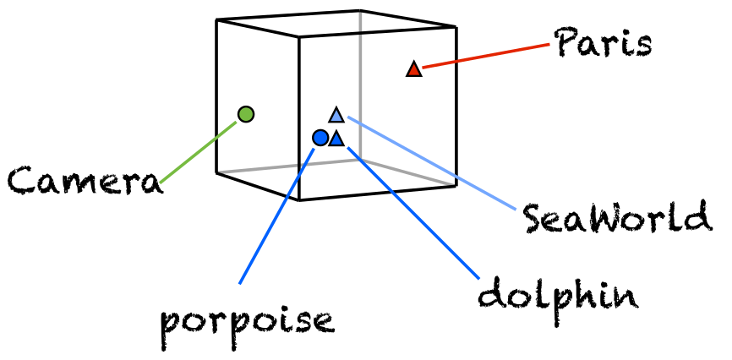
\includegraphics[keepaspectratio,
                     width=.5\paperwidth]{embedding.png}
  \end{center}
  \pause
  \begin{question}
    Как учесть взаимные ссылки между страницами в интернете?
  \end{question}
\end{frame}


\begin{frame}
  \frametitle{Легендарный PageRank}
  \framesubtitle{интуиция}

  Документ $\mathbf{d}$ тем важнее, чем
  \begin{itemize}
    \item больше других документов $\mathbf{c}$ ссылаются на $\mathbf{d}$
    \item важнее эти документы $\mathbf{c}$
    \item меньше других ссылок имеют эти документы $\mathbf{c}$
  \end{itemize}

  \begin{center}
    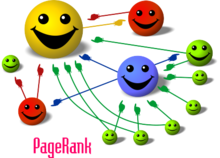
\includegraphics[keepaspectratio,
                     width=.4\paperwidth]{220px-PageRank-hi-res.png}
  \end{center}

  \noindent\rule{8cm}{0.4pt}

  {\it S. Brin, L. Page. The anatomy of a large-scale hypertextual Web search engine. 1998, Computer Networks and ISDN Systems, 30 (1–7): 107–117.}
\end{frame}


\begin{frame}
  \frametitle{PageRank. Формулы}

  Вероятность попасть на страницу $d$, если кликать случайно:

  $$ PR(d) = \frac{1-\delta}{N} + \delta \sum\limits_{c\in D_d^{in}}\frac{PR(c)}{D_c^{out}} $$

  \begin{itemize}
    \item $D_d^{in} \subset D$ — множество документов, ссылающихся на $d$
    \item $D_c^{out} \subset D$ — документы, на которые ссылается $c$
    \item $\delta = 0.85$ — вероятность продолжать клики (damping factor)
    \item $N$ — число документов в коллекции $D$
  \end{itemize}
\end{frame}


\begin{frame}
  \frametitle{PageRank. Теорема Фробениуса-Перрона}

  Матрицу ссылок между сущностями можно представить в виде

  $$ P = \left( \begin{array}{ccc}
  p_{11} & \dots & p_{n1} \\
  \dots & \dots & \dots \\
  p_{1n} & \dots & p_{nn} \\
  \end{array} \right)$$

  где $p_{cd} = \frac{1}{|D_c^{out}|}$ — вероятность перейти с $c$-ой сущности на $d$-ую и $\sum\limits_{i=1}^n p_{ci} = 1$

  Предположим, что все $p_{ij} > 0$, тогда по следствию из теоремы Фробениуса-Перрона существует собственный вектор
  $$ x = \left( \begin{array}{c}
  x_{1} \\
  \dots \\
  x_{n}
  \end{array} \right)$$
  такой что $P \cdot x = x$, тогда PageRank = $x$
\end{frame}


\begin{frame}
  \begin{question}
    Как измерить качество ранжирования?
  \end{question}
\end{frame}


\begin{frame}
   \frametitle{Метрики качества ранжирования 1}

     Пусть $\color{red}{Y = \{0,1\}},\ y(q, d)$ — релевантность

     $a(q, d)$ — искомая функция ранжирования,

     $d_q^{(i)}$ — $i$-й документ по убыванию $a(q, d)$

     {\bf Precision (точность)} — доля релевантных среди первых $n$:

     $$ P_n(q) = \frac{1}{n} \sum\limits_{i=1}^{n} y\left(q, d_q^{(i)}\right) $$

     {\bf Average Precision} — средняя $P_n$ по позициям релевантных документов:

     $$ AP(q) =  \sum\limits_n y\left(q, d_q^{(n)}\right) P_n(q) \big/ \sum\limits_n y\left(q, d_q^{(n)}\right) $$

     {\bf Mean Average Precision} — средняя $AP$ по всем запросам:

     $$ MAP = \frac{1}{|Q|} \sum\limits_{q \in Q} AP(q) $$
\end{frame}


\begin{frame}
  \frametitle{Метрики качества ранжирования 2}

  Пусть $\color{red}{Y \subset \mathbb{R}}, y(q, d)$ — релевантность,

  $a(q, d)$ — искомая функция ранжирования,

  $d_q^{(i)}$ — $i$-й документ по убыванию $a(q, d)$

  \vspace{1cm}
  Доля инверсий порядка среди первых $n$ документов:

  $$ DP_n (q) = \frac{2}{n(n-1)} \sum\limits_{i<j}^n \left[y(q, d_q^{(i)}) < y(q, d_q^{(j)}) \right]$$
\end{frame}


\begin{frame}
  \frametitle{Метрики качества ранжирования 3}

  Пусть $\color{red}{Y \subset \mathbb{R}}, y(q, d)$ — релевантность,

  $a(q, d)$ — искомая функция ранжирования,

  $d_q^{(i)}$ — $i$-й документ по убыванию $a(q, d)$

  {\it Дисконтированная} (взвешенная) сумма выигрышей:

  $$ DCG_n(q) = \sum\limits_{i=1}^n \underbrace{G_q(d_q^{(i)})}_{gain} \cdot \underbrace{D(i)}_{discount}$$

  $G_q(d) = (2^{y(q, d)}-1)$ — больший вес релевантным документам

  $D(i) = 1 / \log_2(i+1)$ — больший вес в начале выдачи

  Нормированная дисконтированная сумма выигрышей:

  $$ NDCG_n(q) = \frac{DCG_n(q)}{\max DCG_n(q)}$$

  $\max DCG_n(q)$ — это $DCG_n(q)$ при идеальном ранжировании
\end{frame}


\begin{frame}
  \frametitle{Подходы к построению моделей ранжирования}

   \begin{itemize}
     \item point-wise — поточечный
     \item pair-wise — попарный
     \item list-wise — списочный
   \end{itemize}
\end{frame}


\begin{frame}
  \frametitle{Pair-wise. RankNet}

  {\bf RankNet}: гладкий функционал качества ранжирования

  $$ Q(a) = \sum\limits_{i \prec j} \mathcal{L}(a(x_j) - a(x_i)) \to \min $$

  при $\mathcal{L}(M) = \log(1 + e^{-\sigma M})$ и линейной модели $a(x) = \left< w, x\right>$

  \vspace{0.5cm}
  {\bf Метод стохастического градиента}:

  выбираем на каждой итерации случайную пару $i \prec j$:

  $$ w := w + \eta \cdot \frac{\sigma}{1 + \exp(\sigma \left< x_j - x_i, w\right>)} \cdot (x_j - x_i)$$

  \noindent\rule{8cm}{0.4pt}

  {\small
  {\it Christopher J.C. Burges.} From RankNet to LambdaRank to LambdaMART: An Overview // Microsoft Research Technical Report MSR-TR-2010-82. 2010.}
\end{frame}


\begin{frame}
  \frametitle{List-wise. От RankNet к LambdaRank}

  {\bf Метод стохастического градиента}:

  $$ w := w + \eta \cdot \frac{\sigma}{\underbrace{1 + \exp(\sigma \left< x_j - x_i, w\right>)}_{\lambda_{ij}} } \cdot (x_j - x_i)$$

  Оказывается для оптимизации негладких функционалов $MAP,\ NDCG,\  pFound$ достаточно домножить $\lambda_{ij}$ на изменение данного функционала при перестановке местами $x_i  \rightleftarrows x_j$

  {\bf LambdaRank}: домножение на изменение $NDCG$ при $x_i  \rightleftarrows x_j$ приводит к её оптимизации

  $$ w := w + \eta \cdot \frac{\sigma}{1 + \exp(\sigma \left< x_j - x_i, w\right>)}\cdot |\Delta NDCG_{ij}| \cdot (x_j - x_i)$$

  \noindent\rule{8cm}{0.4pt}

  {\small
  {\it Christopher J.C. Burges.} From RankNet to LambdaRank to LambdaMART: An Overview // Microsoft Research Technical Report MSR-TR-2010-82. 2010.}
\end{frame}


\begin{frame}
  \frametitle{List-wise. LambdaMART}

  MART (Multiple Additive Regression Trees) = Gradient Boosting

  $$ f_{T, i} := f_{T-1, i} + \alpha b(x_i), i = 1, \dots, \ell $$

  {\bf Идея}: будем искать такой базовый алгоритм $b_T$, чтобы вектор $\left(b_T(x_i)\right)_{i=1}^\ell$ приближал вектор антиградиента $\left(-g_i\right)_{i=1}^\ell$

  $$ b_T := \arg\min\limits_b \sum\limits_{i=1}^\ell \left( b(x_i) + g_i \right)^2$$

  Пусть $\eta_{ij} = \lambda_{ij} \cdot |\Delta NDCG_{ij}|$, пусть $\eta_i = \sum\limits_{(i,j) \in I} \eta_{ij} - \sum\limits_{(j,i) \in I} \eta_{ji}$

  Положим $g_i = \eta_i$

  won Track 1 of the 2010 Yahoo! Learning To Rank Challenge

  \noindent\rule{8cm}{0.4pt}

  {\small
  {\it Christopher J.C. Burges.} From RankNet to LambdaRank to LambdaMART: An Overview // Microsoft Research Technical Report MSR-TR-2010-82. 2010.}
\end{frame}


\begin{frame}
  \frametitle{Рекомендательные системы}

  \begin{center}
    
\includegraphics[keepaspectratio,
                   width=.9\paperwidth]{rec_sys_mem.jpeg}
  \end{center}
\end{frame}


\begin{frame}
  \frametitle{Рекомендательные системы. Постановка задачи}

  $U$ — множество субъектов (users)

  $I$ — множество объектов (items)

  $Y$ — оценки (ratings)

  \vspace{1cm}
  Даны

  $$ (u_t, i_t, y_t) \in D \subset U \times I \times Y $$

  нужно предсказать для $y$ для $(u, i) \notin D$

  \vspace{1cm}
  $ R = (r_{ui})_{U\times I}$ — матрица отношений
\end{frame}


\begin{frame}
  \frametitle{Рекомендательные системы. Пример}

  \begin{center}
    
\includegraphics[keepaspectratio,
                   width=.8\paperwidth]{rec_sys.jpg}
  \end{center}
\end{frame}


\begin{frame}
  \frametitle{Рекомендательные системы. Методы оценки. RMSE}

  $$ \text{RMSE} = \sqrt{\frac{1}{|D^\prime|} \sum\limits_{(u,i) \in D^\prime} (r_{ui}-\hat r_{ui})^2} $$

  \vspace{1cm}
  Исторически она использовалась в легендарном \href{https://ru.wikipedia.org/wiki/Netflix_Prize}{конкурсе Netflix}: 2007 год, \$1 млн

\end{frame}


\begin{frame}
  \frametitle{Корреляционные модели рекомендаций}

  {\bf Подход 1} [оригинально Amazon.com]:

  «клиенты, купившие $i_0$, также покупали $I(i_0)$»

  \vspace{1cm}
  Недостатки:
  \begin{itemize}
    \item рекомендации тривиальны (просто наиболее популярное предлагается)
    \item не учитываются интересы конкретного пользователя $u_0$
    \item проблема «холодного старта» — новый товар никому не рекомендуется
    \item надо хранить всю матрицу $R$
  \end{itemize}

\end{frame}


\begin{frame}

  {\bf Подход 2}:

  «клиенты, похожие на $u_0$, также покупали $I(u_0)$»

  \vspace{1cm}
  \begin{itemize}
   \item \sout{рекомендации тривиальны}
   \item \sout{не учитываются интересы конкретного пользователя $u_0$}
   \item проблема «холодного старта» — новый товар никому не рекомендуется
   \item надо хранить всю матрицу $R$
   \item {\color{gray} нечего рекомендовать нетипичным/новым пользователям}
  \end{itemize}

\end{frame}


\begin{frame}

  {\bf Подход 3}:

   «вместе с объектами, которые покупал $u_0$, часто покупают $I(u_0)$»

   \vspace{1cm}
   \begin{itemize}
    \item рекомендации часто тривиальны (нет коллаборативности)
    \item \sout{не учитываются интересы конкретного пользователя $u_0$}
    \item проблема «холодного старта» — новый товар никому не рекомендуется
    \item надо хранить всю матрицу $R$
    \item \sout{нечего рекомендовать нетипичным/новым пользователям}
   \end{itemize}
\end{frame}


\begin{frame}
  \frametitle{Латентные модели рекомендаций}

  $$ u \to [p_{1u},\dots, p_{tu}, \dots, p_{Tu}] = p_u$$

  $$ i \to [q_{1i},\dots, q_{ti}, \dots, q_{Ti}] = q_i$$

  $$T \ll |U|, T \ll |I|$$

  $ \left<p_u, q_i\right> = \sum\limits_{t=1}^T p_{tu} q_{ti} $ — рейтинг i-го объекта для u-ого субъекта
\end{frame}


\begin{frame}
  \frametitle{Singular Value Decomposition (SVD-разложение)}

  $ R = P^T \Delta Q$ — матрица рейтингов

  $$ \|R -  P^T \Delta Q\|^2 \to \min\limits_{P, \Delta, Q} $$

  Матрицы $P$ и $Q$ должны быть ортогональны, но на практике это может нам мешать.
\end{frame}


\begin{frame}
  \frametitle{Модель латентных факторов (LFM)}

  \begin{align*}
   J(\Theta) &= \sum\limits_{(u,i) \in D} \left( r_{ui} - \overline r_{u} - \overline r_{i} - \sum\limits_{t \in T} p_{tu}q_{ti}\right)^2 \to \min\limits_{P, Q} \\
  p_{tu} &= p_{tu} + \eta \varepsilon_{ui}q_{ti}, t \in T \\
  q_{ti} &= q_{ti} + \eta \varepsilon_{ui}p_{tu}, t \in T
  \end{align*}

  $\overline r_{u}$ — усреднение по оценкам пользователя (есть восторженные, у которых оценки рейтинга это 4 и 5, есть наоборот ставящие только 1 и 3 из 5)

  $\overline r_{i}$ — аналогично по объектам (сложно ненавидеть котика)
\end{frame}


\begin{frame}
  \frametitle{Модель латентных факторов (LFM). Достоинства}

  легко вводится регуляризация:

  $$ \varepsilon^2_{ui} + \lambda \|p_u\|^2 + \mu \|q_i\|^2 \to \min\limits_{p_u, q_i}$$

  легко вводятся ограничения неотрицательности:

  $ p_{tu} \geq 0, q_{ti} \geq 0 $ (метод проекции градиента)

  легко вводится обобщение для ранговых данных:

  $$ \sum\limits_{(u,i) \in D} \left(r_{ui} - \overline r_{u} - \overline r_{i} - \color{red}{\beta} \left(\sum\limits_{t \in T} p_{tu}q_{ti} \right) \right)^2 \to \min\limits_{P, Q, \color{red}{\beta}}$$

  легко реализуются добавления ещё одного:
  \begin{itemize}
   \item клиента $u$
   \item объекта $i$
   \item значения $r_{ui}$
  \end{itemize}

   высокая численная эффективность на больших данных
\end{frame}


\begin{frame}
  \frametitle{Alternating Least Squares (ALS)}

  Попеременно точно (аналитически) находим минимумы то по одним координатам, то по другим:

  $$ p_u^* (\Theta) = \arg\min\limits_{p_u} J(\Theta) = \left(Q_u^TQ_u + \lambda I \right)^{-1} Q_u^T r_u$$

  $$ q_i^* (\Theta) = \arg\min\limits_{q_i} J(\Theta) = \left(P_i^TP_i + \lambda I \right)^{-1} P_i^T r_i$$

  Работает достаточно быстро, так как каждый шаг можно распараллелить. Используется в известном фреймворке Spark обработки больших данных от Apache.
\end{frame}


\begin{frame}
  \frametitle{Учет неявной информации}

  Пусть имеются

  $r_{ui}$ — явные оценки (explicit)

  $s_{ui}$ — неявные оценки (implicit)

  Пусть $c_{ui} = 1 + \alpha r_{ui}$ — взвешиваем имеющимися явными оценками

  $$ \hspace{-0.5cm} \sum\limits_{(u,i) \in D} c_{ui} \left(s_{ui} - \overline s_u - \overline s_i - \sum\limits_{t \in T} p_{tu}q_{ti} \right)^2   + \lambda \sum\limits_{u \in U} \|p_u \|^2 + \mu \sum\limits_{i \in I} \|q_i \|^2 \to \min\limits_{P, Q}$$

  \vspace{1cm}
  \noindent\rule{8cm}{0.4pt}

  {\small
  {\it Bell R.M., Koren Y., Volinsky C.} The BellKor 2008 solution to the Netflix Prize.}

\end{frame}


\begin{frame}
  \frametitle{Метрики в рекомендательных системах}

  Недостатки RMSE:
  \begin{itemize}
    \item у каждого пользователя свое представление о шкале оценок. Пользователи, у которых разброс оценок более широкий, будут больше влиять на значение метрики, чем другие
    \item Ошибка в предсказании высокой оценки имеет такой же вес, что и ошибка в предсказании низкой оценки. При этом в реальности предсказать оценку 9 вместо настоящей оценки 7 страшнее, чем предсказать 4 вместо 2 (по десятибалльной шкале)
    \item Можно иметь почти идеальную метрику RMSE, но иметь очень плохое качество ранжирования, и наоборот
  \end{itemize}

  Часто лучше использовать метрики ранжирования:
  \begin{itemize}
   \item MAP
   \item NDCG
  \end{itemize}
\end{frame}


\begin{frame}
  \frametitle{Нетривиальные метрики качества}

  Другие свойства рекомендаций, влияющие на качество.

  \vspace{0.5cm}
  Для пользователя:
  \begin{itemize}
    \item разнообразие (diversity)
    \item неожиданность (surprise)
    \item новизна (novelty)
    \item догадливость (serendipity)
  \end{itemize}

  \vspace{0.5cm}
  Для бизнеса:
  \begin{itemize}
    \item покрытие (coverage)
    \item заинтересованность в платформе
  \end{itemize}
\end{frame}


\begin{frame}
  \frametitle{Bayesian Personalized Ranking (BPR)}

  На входе
  \begin{itemize}
    \item по сути только факт взаимодействия пользователь-объект
    \item Нет дизлайков :)
  \end{itemize}

  \begin{center}
    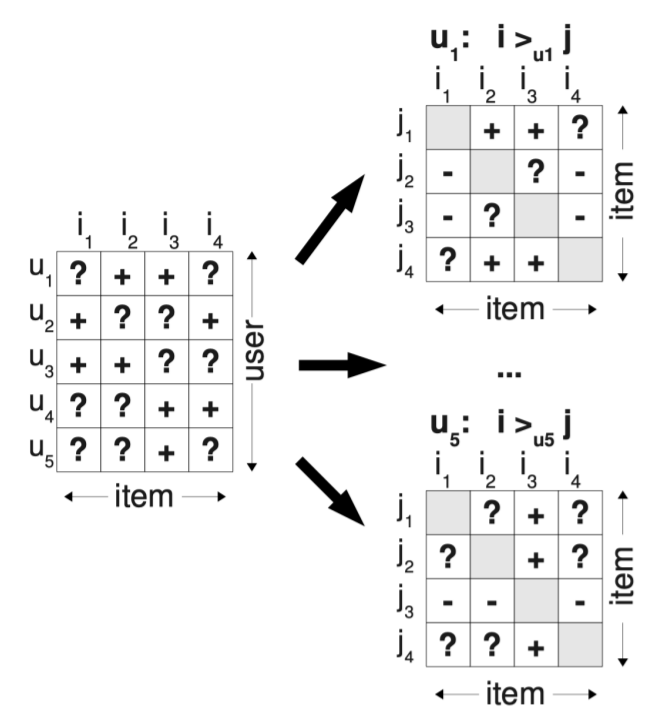
\includegraphics[keepaspectratio,
                     width=.4\paperwidth]{BPR.png}
  \end{center}

  $D_S = \{(u,i,j) | i \in I_u^+ \wedge j \in I \backslash I^+_u \}$
\end{frame}


\begin{frame}
  $ p(\Theta | >_u) \propto p(>_u | \Theta) p(\Theta) $

  \begin{align*}
    &\prod\limits_{u \in U} p(>_u | \Theta) = \\
    &= \prod\limits_{(u,i,j) \in U\times I\times I} p(i >_u j | \Theta)^{\delta((u,i,j) \in D_S)}\cdot(1-p(i >_u j | \Theta))^{\delta((u,j,i) \notin D_S}) = \\
    &=\text{\{так как по всем парам сумма\}} \\
    &= \prod\limits_{(u,i,j) \in D_S} p(i >_u j | \Theta)
  \end{align*}

  \begin{align*}
     &p(i >_u j | \Theta) = \sigma(\hat x_{uij}(\Theta)) \\
    \hat x_{uij} &= \hat x_{ui} - \hat x_{uj} = \hat r_{ui} - \hat r_{uj} \\
    \sigma(x) &= \frac{1}{1 + e^{-x}}
  \end{align*}

  Оптимизация привычным градиентным спуском.

  \noindent\rule{8cm}{0.4pt}

  {\small
  {\it Rendle, Freudenthaler, Gantner and Schmidt-Thieme.} BPR: Bayesian Personalized Ranking from Implicit Feedback.}
\end{frame}


\begin{frame}
  \frametitle{BPR (Bayesian Personalized Ranking). Достоинства}

  \begin{itemize}
    \item разумный учет неявного фидбека
    \item ориентированность на ранжирование
  \end{itemize}
  \pause
  \begin{question}
    Как быть с новыми пользователями и объектами?
  \end{question}
  \pause
  {\bf Вариант 1}. Обучаем модель предсказывать скрытое состояние по пользователю.

  {\bf Вариант 2}. (для объектов) Многорукие бандиты — с некоторой вероятностью показываем каждый новый объект пользователю и пересчитываем вероятности, накапливая статистику взаимодействия.
\end{frame}


\begin{frame}
  \frametitle{Как обычно происходит на практике?}

  \begin{enumerate}
    \item Сначала происходит быстрая генерация кандидатов (например, \href{https://github.com/facebookresearch/faiss}{https://github.com/facebookresearch/faiss})
    \item После этого применяется более тяжелая и точная ранжирующая модель
  \end{enumerate}
\end{frame}


\begin{frame}
  \frametitle{Резюме}

  \begin{itemize}
    \item постановка задачи ранжирования, возможные метрики
    \item подходы к построению моделей ранжирования: поточечный, попарный, списочный
    \item SVD, LFM, ALS
    \item BPR
  \end{itemize}

  \pause
  \vspace{1cm}
  Что ещё можно посмотреть?
  \begin{itemize}
    \item \href{https://youtu.be/2F5kTOiDuOg}{Доклад} про рекомендации ленты ВКонтакте на Open DataFest 2020
    \item \href{https://www.youtube.com/watch?v=oavkOOJMVK8}{Рекомендательная система на базе DataSphere}
  \end{itemize}
\end{frame}

\end{document}
